\RequirePackage[l2tabu, orthodox]{nag}
% \RequirePackage{silence}
  % \WarningFilter{nag}{Command}

\documentclass[letterpaper]{article}

\usepackage[numbers]{natbib}

%%% Subliminal refinements towards typographical perfection (1%)
\usepackage[stretch=10]{microtype}

%%% Handle input and output of accented/special characters and modern fonts
\usepackage[T1]{fontenc}
\usepackage[utf8]{inputenc}
\usepackage{lmodern}

\usepackage[american]{babel}
\usepackage{csquotes}


%%% Better biblatex
% \let\citename\relax
% \usepackage[style=ACM-Reference-Format,
%   abbreviate=true, dateabbrev=true, isbn=true, doi=true, urldate=comp, url=true, eprint=false,
%   maxbibnames=9, minbibnames=9, maxcitenames=1, mincitenames=1,
%   backref=false, backend=biber, language=american, sortcites=true,
%   autocite=inline% , labelnumber=true
%   ]{biblatex}
% % \cite, \parencite, \footcite, \textcite, \autocite

% \setcounter{biburlnumpenalty}{100}
% \setcounter{biburllcpenalty}{9000}

% \addbibresource{references/refs.bib}
% \renewcommand{\bibfont}{\Small}

%%% Include todo notes while writing draft (\listoftodos, \todo, \missingfigure)
\usepackage[color=white]{todonotes}

%%% Demo boxes
\usepackage{xcolor}
\newcommand\crule[3][black]{\textcolor{#1}{\rule{#2}{#3}}}

%%% Easier SI units
\usepackage[allowlitunits]{siunitx}

%%% Improved subfigures
\usepackage[caption=false,font=footnotesize]{subfig}
\usepackage[export]{adjustbox}

%%% Better looking tables
\usepackage{booktabs}
\renewcommand{\arraystretch}{1.2}
\usepackage{array}

%%% Better handling of links
\usepackage{url}

%%% Better math
\usepackage{amsmath}

%%% Internal references
\usepackage{hyperref}


%%% Colors for tracking changes
\newcommand{\red}[1]{\textcolor{red}{#1}}
\newcommand{\blue}[1]{\textcolor{blue}{#1}}

% \usepackage{setspace}
% \doublespacing


%%% Commands for easily changing formatting (e.g., italicize)
\newcommand{\etal}{et~al.}
\newcommand{\ie}{i.e.}
\newcommand{\eg}{e.g.}

\newcommand{\figref}[1]{Figure~\ref{#1}}
\newcommand{\tblref}[1]{Table~\ref{#1}}
\newcommand{\secref}[1]{Section~\ref{#1}}


\title{Evolving Controllers for a Transformable Wheel Mobile Robot}

\author{Anthony J. Clark,$^{1}$ Keith A. Cissell$^{1}$, and Jared M. Moore$^{2}$\\
\mbox{}\\
$^1$Missouri State University, Springfield, Missouri, USA\\
$^2$Grand Valley State University, Allendale, Michigan USA\\
AnthonyClark@MissouriState.edu}

\begin{document}

\maketitle

% Maximum 200 words

\begin{abstract}

%%% Background
% This section should be the shortest part of the abstract and should very briefly outline the following information:
% - What is already known about the subject, related to the paper in question
% - What is not known about the subject and hence what the study intended to examine (or what the paper seeks to present)
Unmanned ground vehicles (UGVs) are well suited to tasks that are either too dangerous or too monotonous for people. For example, UGVs can traverse arduous terrain in search of disaster victims.
%
However, it is difficult to design these system so that they perform well in a variety of different environments.
%
%
%
%%% Methods
% The methods section is usually the second-longest section in the abstract. It should contain enough information to enable the reader to understand what was done, and how.
In this study, we evolve controllers and physical characteristics of a UGV with transformable wheels to improve its mobility in a simulated environment.
%
The UGV's mission is to visit a sequence of coordinates while automatically handling obstacles of varying sizes by extending wheel struts radially outward from the center of each wheel.
%
Evolved finite state machines (FSMs) and artificial neural networks (ANNs) are compared, and a set of controller design principles are gathered from analyzing these experiments.
%
%
%
% Results
% The results section should be the longest part of the abstract and should contain as much detail about the findings as the journal word count permits.
%
Results show comparable performance between FSM and ANN controllers, but the evolved strategies differ.
%
% The final controller is designed to take advantage of both approaches: (1) the control system is no longer a black-box and can be predictably understood (unlike the ANN), and (2) it takes advantage of the continuous nature of an ANN.
%
%
%
% Conclusion
% This section should contain the most important take-home message of the study, expressed in a few precisely worded sentences. Usually, the finding highlighted here relates to the primary outcome measure; however, other important or unexpected findings should also be mentioned. It is also customary, but not essential, for the authors to express an opinion about the theoretical or practical implications of the findings, or the importance of their findings for the field. Thus, the conclusions may contain three elements:
% - The primary take-home message
% - The additional findings of importance
% - The perspective
% UGVs are valuable in many domains, however, they must be designed to work in many different environments.
%
Furthermore, we show that a UGV's controller and physical characteristics can be effectively chosen by examining results from evolutionary optimization.

\end{abstract}




% Unmanned ground vehicles (UGVs) are well suited to tasks that are either too dangerous or too monotonous for people. For example, UGVs can traverse arduous terrain in search of disaster victims. However, it is difficult to design these system so that they perform well in a variety of different environments. In this study, we evolve controllers and physical characteristics of a UGV with transformable wheels to improve its mobility in a simulated environment. The UGV's mission is to visit a sequence of coordinates while automatically handling obstacles of varying sizes by extending wheel struts radially outward from the center of each wheel. Evolved finite state machines (FSMs) and artificial neural networks (ANNs) are compared, and a set of controller design principles are gathered from analyzing these experiments. Results show comparable performance between FSM and ANN controllers, but the evolved strategies differ. Furthermore, we show that a UGV's controller and physical characteristics can be effectively chosen by examining results from evolutionary optimization.


% \keywords{evolutionary robotics, artificial neural network, finite state machine, adaptive, unmanned ground vehicle}

% TODO:
% - compare final results with novel environment (different way-points)
% - textit vs emph vs mathit


\section{Introduction}


% (1) Introductory paragraph: Very briefly: What is the problem and why is it relevant to the audience attending *THIS CONFERENCE*? Moreover, why is the problem hard, and what is your solution? You must be brief here. This forces you to boil down your contribution to its bare essence and communicate it directly.
Autonomous unmanned ground vehicles (UGV) provide an excellent solution to tasks that require searching or monitoring in environments deemed too remote or dangerous for humans.
%
Consider \emph{search and rescue}: after a natural disaster a UGV can be used by first responders to help locate victims in unstable and hazardous locations.
%
% Compared with an unmanned aerial vehicle (UAV), a
UGVs have long operating durations, can carry heavy payloads (\eg{}, sensors), and can search in narrow and covered places such as forests and caves.
%
% Ideally, a heterogeneous swarm of UAVs and UGVs would coordinate to gain the advantages of both search modes~\citep{Kruijff.SearchAndRescue.ICFSR.2014}.
%
% In this paper, however, we limit our investigation to UGVs.
% In particular, we show results for improving the mobility of Adabot, a UGV that includes wheel struts.


% (2) Background paragraph: Elaborate on why the problem is hard, critically examining prior work, trying to tease out one or two central shortcomings that your solution overcomes.
% One issue that arises during the design of a UGV is how to ensure that the system
Ensuring that a UGV can handle many different types of terrain is an ongoing challenge.
%
Researchers have invented several different methods for addressing the issue of mobility in varied terrain.
%
Specifically, robots have been designed with treaded wheels, tracks, legged-wheels (wheels are rimless, wheel spokes make contact with the ground), wheeled-legs (wheels are on the end of legs and the suspension is potentially actively actuated), and transformable wheels~\citep{Saranli.IntJrnRoboRes.RHex.2001,Quinn.IROS.Whegs.2002,Eich.SSRR.Stair-climb-SAR.2008,Haldane.ICRA.VelociRoACH.2013,Kenneally.IEEERobAutLetters.Legged-robots.2016}.
%
Although these systems provide an advantage over traditional wheeled robots, optimization is not performed in the vast majority of these studies.
%
% \blue{How could EA help?}


% (3) Transition paragraph: What keen insight did you apply to overcome the shortcomings of other approaches? Structure this paragraph like a syllogism: Whereas P and P => Q, infer Q.
The device in this study, the \emph{Adabot} (see \figref{fig:adabot}), includes transformable wheels that can smoothly be converted from a round wheel, to a wheel with tire \emph{studs}, to a legged-wheel.
%
Wheel transformations are performed by extending wheel struts radially outward from the center of the wheel (see \figref{fig:wheel-extender}).
 % (see \secref{sec:adabot} for details \ref{sec:adabot} \nameref{sec:adabot}).
%
Adabot has been optimized using an evolutionary algorithm such that its physical characteristics and its controller are better able to handle terrain that includes obstacles of varying sizes.
%
In previous work~\citep{Clark.2017.SSCI.Adabot}, a similar system was optimized to maximum forward velocity over uneven terrain.
%
The present study differs in two main ways: (1) here we evolve controllers for a more difficult task: \emph{way-point following}, and (2) we analyze results from evolving two controller types of feedback controllers (rather than feed-forward).



% (4) Details paragraph: What technical challenges did you have to overcome and what kinds of validation did you perform?
In this study, we evolve the robot's chassis dimensions, its wheel radius, the number of wheel struts,
% (described in \secref{sec:adabot}),
along with either a finite state machine (FSM) controller or an artificial neural network (ANN) controller.
%
The best evolved FSMs and ANNs are analyzed and compared.
%
For this initial work, to ensure that we are able to effectively analyze the ANN, the network only has three input nodes, zero hidden nodes, and three output nodes. The inputs are fully connected to the outputs.
%
The network is only slightly more complex than a Type 2 Braitenberg vehicle~\citep{Braitenberg.Vehicles.Book.1986}.
%
Conclusions drawn from our analysis are used to create a set of design principles for a new controller that takes advantage of both techniques.
%
In particular, it is attractive to design a controller that is not a black-box like an ANN but less rigidly defined than an FSM.
%
% \blue{hybrid controller}
%
%
% (5) Assessment paragraph: Assess your results and briefly state the broadly interesting conclusions that these results support. This may only take a couple of sentences. I usually then follow these sentences by an optional overview of the structure of the paper with interleaved section callouts.
% The results presented in this study demonstrate how a UGV can be optimized to improve robustness.
%
% Specifically, evolving Adabot has made it more robust in the presence of varied terrain.
%
% The techniques and concepts presented in this study can be applied to the optimization of any physical system.
%
Source code has been made available on GitHub\footnote{\url{https://github.com/anthonyjclark/adabot02-ann}}.

% \vspace{-0.1in}

\begin{figure}[!ht]
    \centering

    % \subfloat[]{\fbox{\crule[white]{0.4\columnwidth}{2cm}}}
    % \hfil
    % \subfloat[]{\fbox{\crule[white]{0.4\columnwidth}{2cm}}}

    \subfloat[3D Printed Prototype]{%
        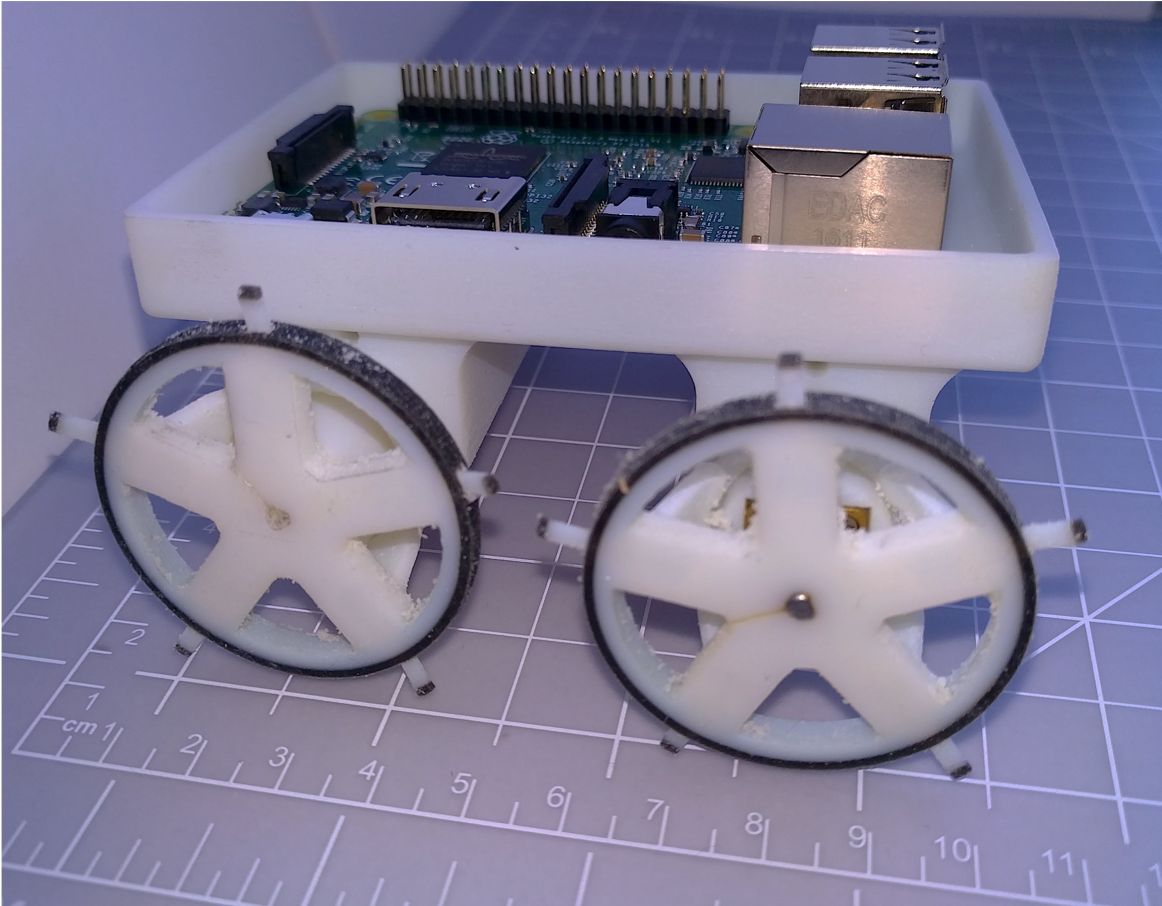
\includegraphics[width=0.2\textwidth,valign=c]{figures/1-introduction/perspective-image.jpg}%
    }\quad
    \subfloat[Simulated Device]{%
        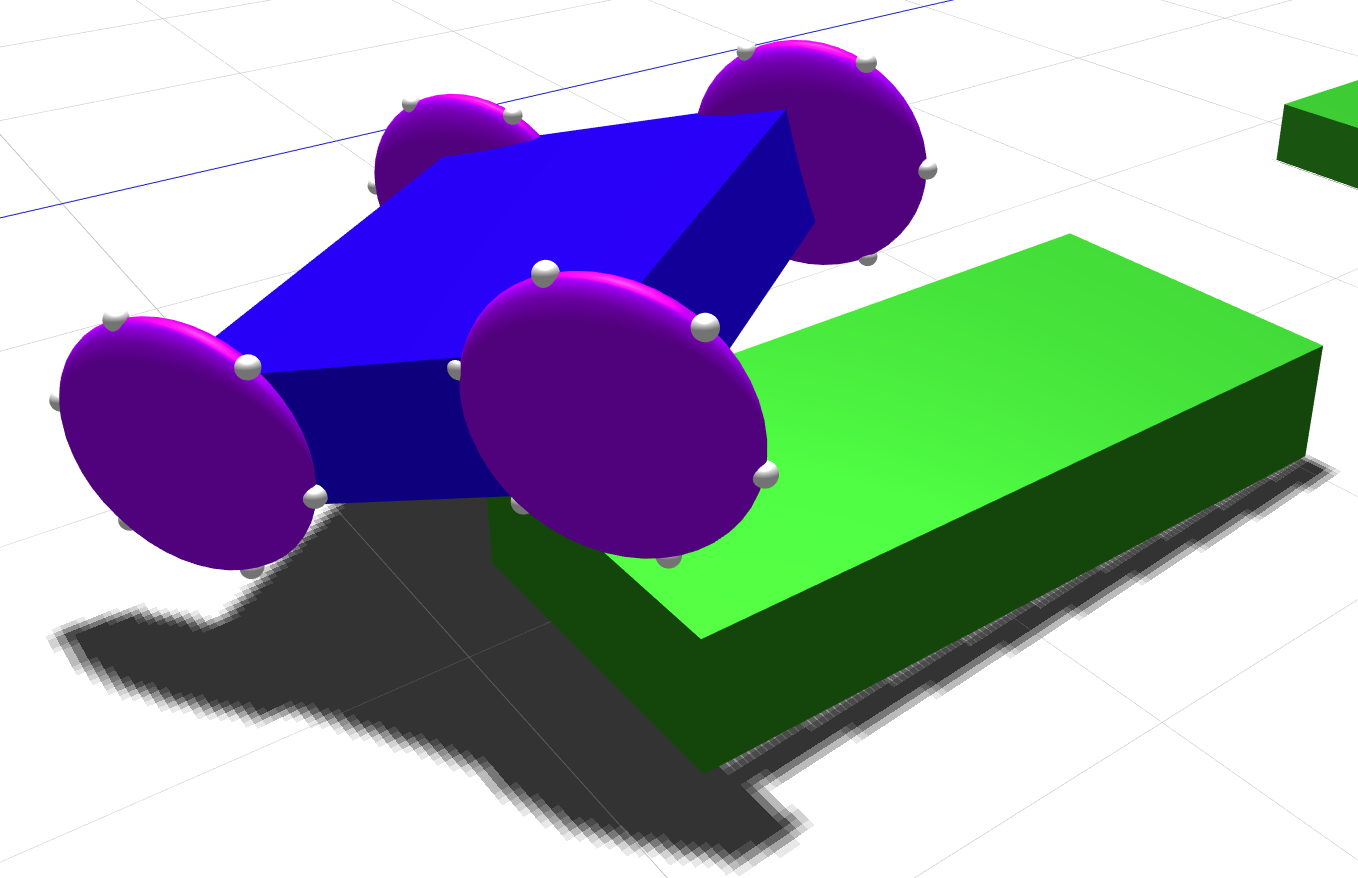
\includegraphics[width=0.2\textwidth,valign=c]{figures/1-introduction/simulation-climbing.png}%
        \vphantom{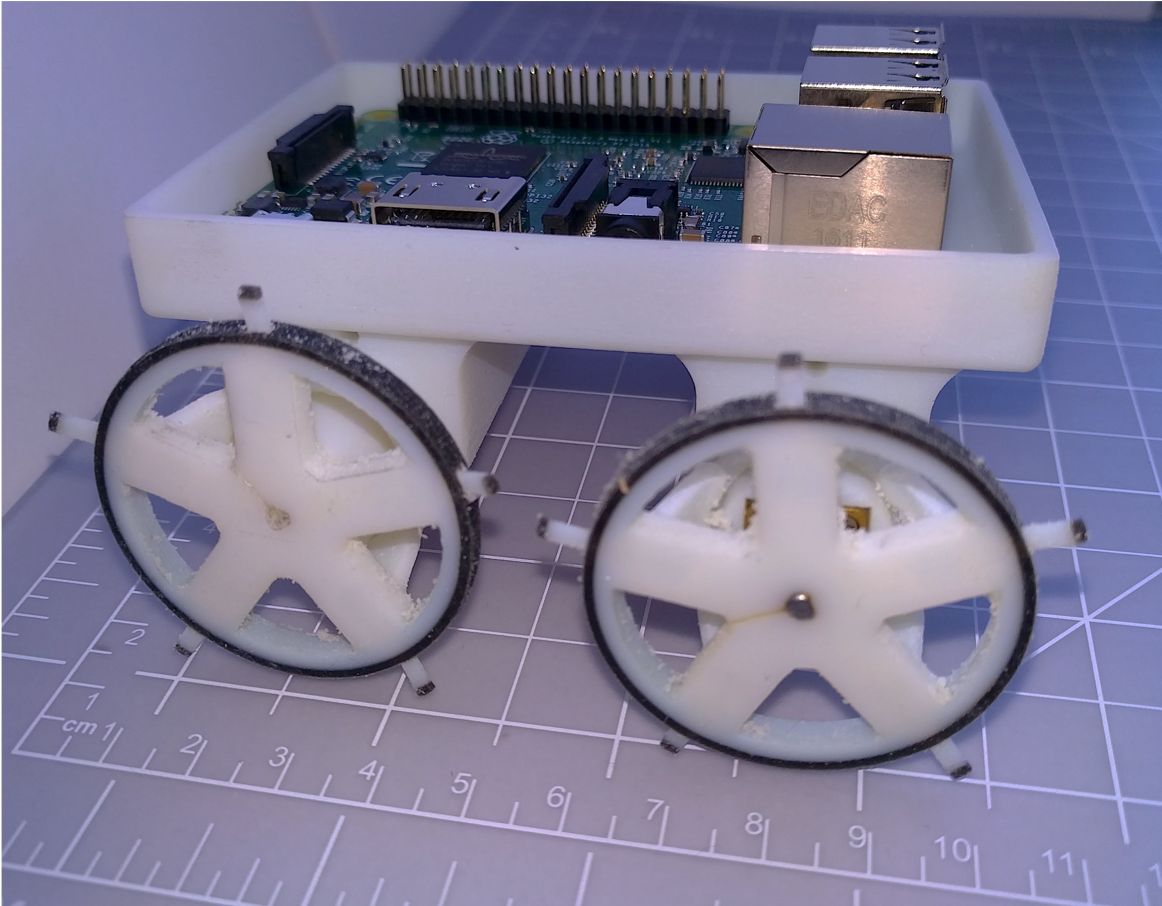
\includegraphics[width=0.2\textwidth,valign=c]{figures/1-introduction/perspective-image.jpg}}%
    }

    \vspace{-0.05in}

    \caption{Adabot, a UGV with transformable wheels.}
    \label{fig:adabot}

    \vspace{-0.15in}

\end{figure}

% \vspace{-0.1in}

\section{Related Work}
\label{sec:related-work}

% \red{Robots are well suited to tasks that are too mundane, precise, or dangerous for humans.
% %
% Increasingly, autonomous robots are being developed to operate in rugged and dynamic environments.
% %
% Such terrain is particularly difficult for wheeled UGVs, which has prompted the design of many different suspensions and wheel configurations~\citep{Seeni.Mobility.InTech.2010}.
% %
% The challenge for these devices is to successfully navigate an area without prior knowledge of the obstacles and ground consistency.
% %
% Moreover, robotics engineers must choose values for all free parameters (\eg{}, the chassis and wheel dimensions).}


% Evolve UGVs (ER)
In the field of evolutionary robotics (ER), an evolutionary algorithm (EA) optimizes free variables of a given system~\citep{Silva.EvolComp.Issues-ER.2016}.
%
ER methods have been successfully applied to many different types of robotic systems (aerial, aquatic, walking, etc.).
%
% TODO change this citation
For example, we have previously used differential evolution to evolve an adaptive neural network for a robotic fish \citep{Clark.GECCO.MFAC.2015}, and \citet{Moore.2017.GECCO.Animat} evolved hierarchical controllers for segmented worm-like animats.
%
Although evolution has been regularly utilized at an abstract level to optimize wheeled-robot navigation processes (for example, see~\citet{Gomes.2015.GECCO.Maze}), it has not often been used to directly evolve UGVs, and to the best of our knowledge this is the first study in which the characteristics of a transformable wheel are evolved.
%
% However, as identified by \citet{Bongard.2013.CACM.ER}, and in the work presented here, ER methods can be effectively applied to wheeled robots.


% Analyze neural networks
A large number of ER studies utilize ANNs to control mobile robots, including \emph{Evolving Virtual Creatures} \citep{Sims.1994.CGIT.Creatures}, which is considered one the the first ER works.
%
ANNs  provide several benefits when using an evolutionary method.
%
First, since ANNs are so-called universal approximators~\citep{Hornik.1989.NN.UniversalANN}, evolution often produces \emph{novel} and sometimes unintuitive results that may not have been found when creating a controller by hand~\citep{Bongard.2013.CACM.ER}.
%
And second, ANNs require a minimal amount of user design. Specifically, an evolutionary algorithm can automatically decide the importance of each input (sensor values) in the calculation of each output (actuation mechanisms)~\citep{Stanley.2002.EC.NEAT}.
%
The primary disadvantage of using an ANN is that it is considered a black-box system. That is, \emph{how} an ANN achieves its results is not often clear or analyzed.
%
Recently, however, some researchers have attempted to extract state machines from evolved neural networks.
%
For example, \citet{Wrobel.2017.SSCI.VSSNN} automatically generated a state machine with the same properties of an evolved spiking neural network.

\section{Adabot}
\label{sec:adabot}

In this section, we describe the prototype Adabot hardware, including the transformable wheel mechanism, along with the simulation environment utilized during evolutionary optimization.

% Hardware
% \subsection{Hardware}
% \paragraph{Hardware}
\vspace{0.1in}
\noindent
\textbf{Hardware}
%
The Adabot, pictured in \figref{fig:adabot}, is a prototype device that includes a Raspberry Pi 3 Model B (RPi) as its main control board.
%
The RPi was chosen for its ability to run the Robot Operating System (ROS)~\autocite{Quigley.ICRAOSS.ROS.2009}, which Adabot uses to manage its software systems.
%
The size of an RPi constrains the minimum dimensions of the Adabot's chassis. Specifically, the chassis must be at minimum 8~\si{cm} by 8~\si{cm}.
%
\tblref{tbl:params-physical} lists all configurable parameters for Adabot's physical characteristics, where
$\mathit{WheelBase}$ and $\mathit{TrackWidth}$ denote the distance between the front and rear axles and the lateral distance between wheels, respectively, and $\mathit{StrutCount}$ parameter indicates the number of struts per wheel.

\begin{table}[hb]
    \centering
    \caption{Adabot Physical Parameters}
    \label{tbl:params-physical}
    \begin{tabular}{@{}ll@{}}
        \toprule
        \textbf{Name} & \textbf{Range}\\
        \midrule
        $\mathit{WheelBase}$    & \numrange{8}{16}~\si{cm}\\
        $\mathit{TrackWidth}$    & \numrange{8}{16}~\si{cm}\\
        $\mathit{WheelRadius}$ & \numrange{2}{3}~\si{cm}\\
        $\mathit{StrutCount}$        & \numrange{0}{7}\\
        \bottomrule
    \end{tabular}
\end{table}



Each of the four wheels is driven by its own DC gear-motor with magnetic encoders.
%
Likewise, each wheel includes a set of struts that can be extended and retracted by a linear servo.
%
For sensing, Adabot includes three forward facing distance sensors and an IMU (3-axis gyroscope, 3-axis accelerometer, and 3-axis magnetometer).
%
Finally, it uses a 2.4 GHz wireless communication module and is powered by a 2200 mAh battery pack, which provides roughly two hours of operating time.


% Extension
% \subsection{Extender Mechanism}
% \paragraph{Extender Mechanism}
\vspace{0.1in}
\noindent
\textbf{Strut Extension}
%
\figref{fig:wheel-extender} depicts the strut extension process.
%
This mechanism enables the wheel to exhibit a range of characteristics.
%
With the struts fully retracted, the wheels operate conventionally; when extended a small amount the struts act as tire studs; and with the struts fully extended each wheel resembles a legged-wheel.
%
The radius of the wheel and the number of struts are both free parameters that can be evolved during optimization.
%
For the following discussion, the most important aspect of this mechanism is that the maximum extension of the struts is equal to 1~\si{cm} minus the wheel's radius ($\mathit{MAXEXT} = \mathit{WheelRadius} - 1~\si{cm}$).
%
For a more detailed discussion of Adabot's software and wheel extension mechanism, and an example of evolving Adabot with ROS and Gazebo (a simulation environment tightly coupled with ROS)~\parencite{Koenig.IROS.Gazebo.2004} see our preliminary study~\red{<citation removed to preserve anonymity>}.



\begin{figure}[!ht]
    \centering

    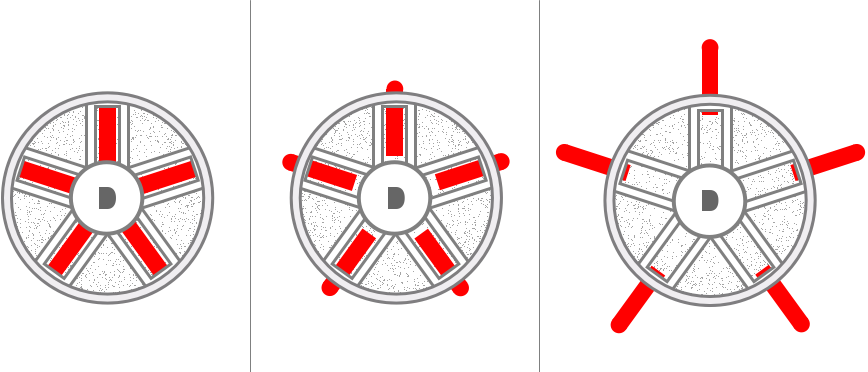
\includegraphics[width=\columnwidth]{figures/3-adabot/extension-mechanism.png}
    % \fbox{\crule[white]{\columnwidth}{2cm}}

    \vspace{-0.08in}

    \caption{An illustration of the Adabot's wheel extension mechanism, where the struts are fully retracted (left), partially extended (middle), and fully extended (right).}
    \label{fig:wheel-extender}

    \vspace{-0.15in}

\end{figure}

% Simulation
% \subsection{Simulation}
% \paragraph{Simulation}
\vspace{0.1in}
\noindent
\textbf{Simulation}
%
% As is the case for most ER studies, we use simulation during the optimization process.
%
An image of the simulation environment is shown in \figref{fig:simulation-environment}.
%
% To populate the environment with obstacles, we generate 40 boxes with random dimensions, positions, and densities.
The environment is populated by generating 40 boxes with random dimensions, positions, and densities.
%
If a newly generated box collides with another box it is removed from the simulation. We see on average 31 boxes in the environment.
%
Box heights are in the range \numrange{2}{5}~\si{cm}, which is high enough compared to the potential $\mathit{WheelRadius}$ values that most traditional wheeled robots will have difficulty climbing them~\autocite{Quinn.IROS.Whegs.2002}.
%
Moreover, rather than each box being in a fixed position, it is possible for the Adabot to push a box (depending on its size and density).


For this study, we are using the Dynamic Animation and Robotics Toolkit (DART)\footnote{https://dartsim.github.io/index.html}.
%
DART is specifically designed for robotics applications (unlike the Open Dynamics Engine\footnote{https://bitbucket.org/odedevs/ode}, which we've used in the past), and is comparable in speed (if not faster) than common alternatives~\autocite{Mouret.2017.SimER.Simulation}.
%
In this study, we do not simulate noise, and we assume that the robot has direct access to its global position and rotation. Essentially, we are mimicking a lab setup with an overhead camera that communicates directly with the robot.


\begin{figure}[!ht]
    \centering

    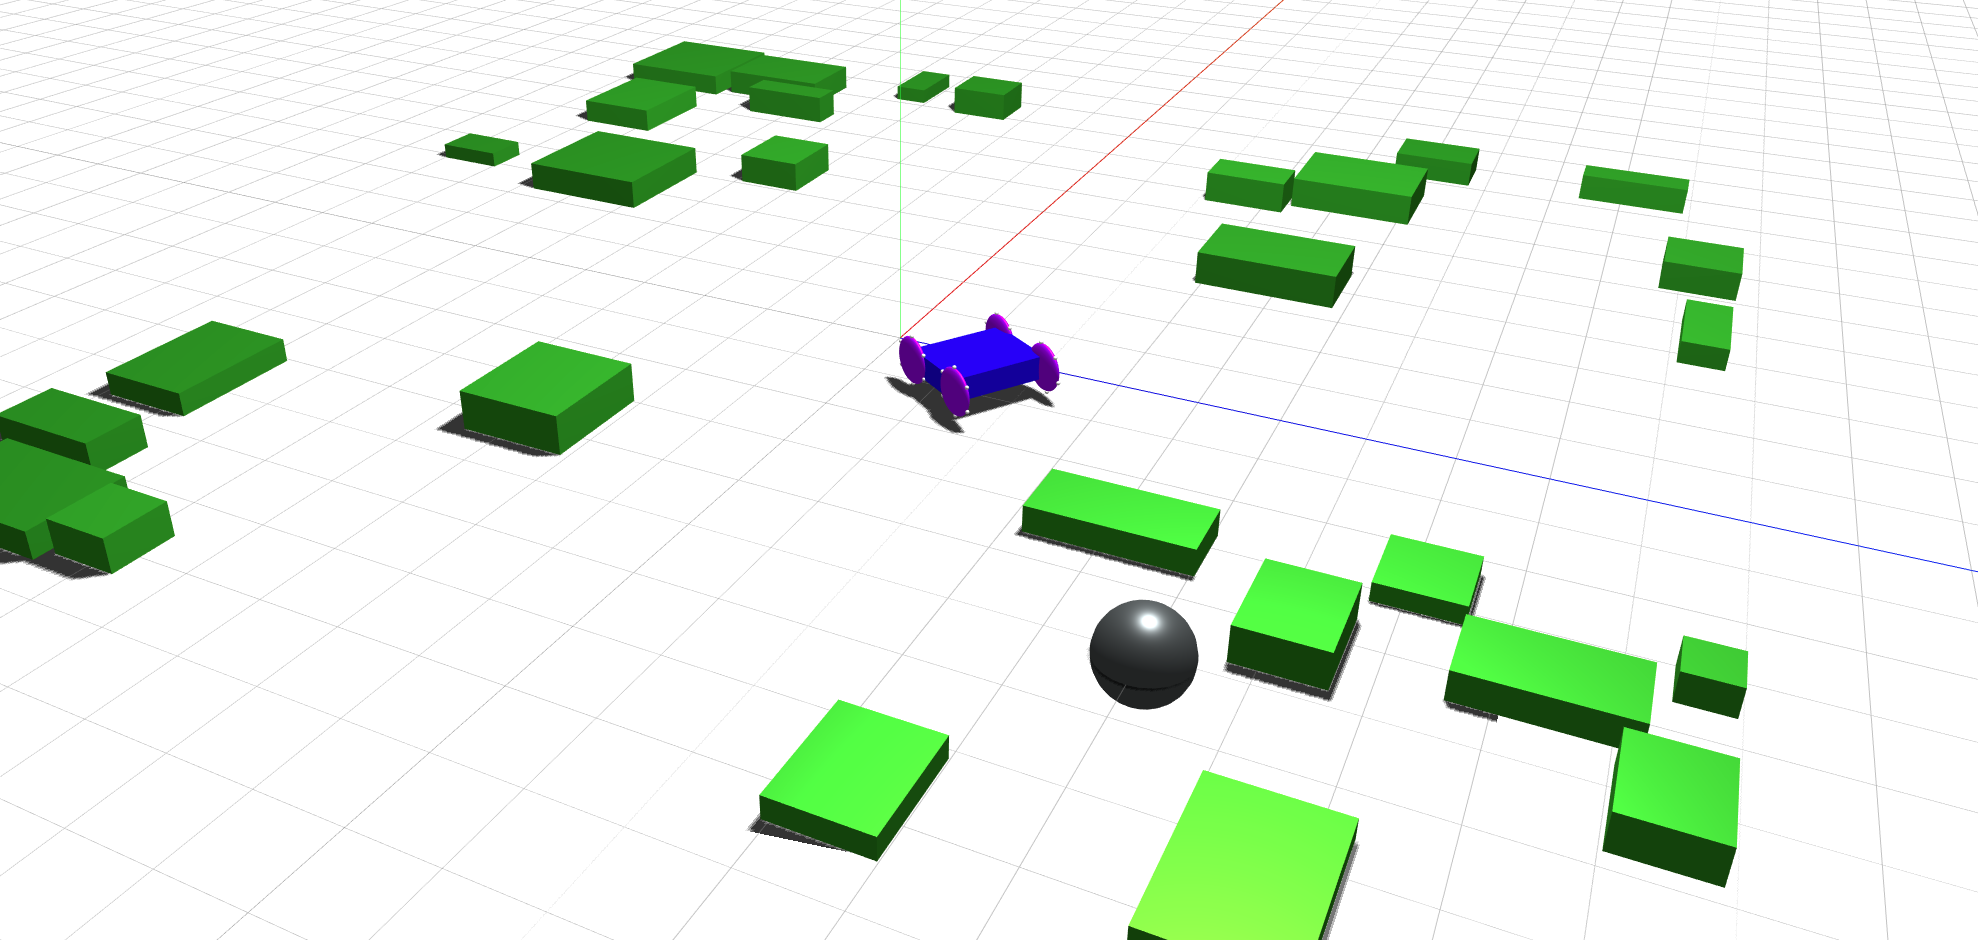
\includegraphics[width=0.8\columnwidth]{figures/3-adabot/environment.png}
    % \fbox{\crule[white]{\columnwidth}{2cm}}

    \vspace{-0.1in}

    \caption{An example environment including randomly generated obstacles. The current way-point is shown in dark gray, and the robot starts at the origin facing in the positive x-axis (away from the way-point, along the red axis line).}
    \label{fig:simulation-environment}

    \vspace{-0.2in}

\end{figure}

% Control Properties
% \subsection{Way-Point Navigation Control}
% \paragraph{Way-Point Navigation Control}
\vspace{0.1in}
\noindent
\textbf{Way-Point Navigation Control}
%
Adabot is a skid-steer style robot--it turns by rotating its left and right wheels at different rates. Although each wheel (and wheel strut set) can be controlled independently, in this study we only have three control outputs: (1) an angular rate for the left wheels, (2) and angular rate for the right wheels, and (3) a single extension amount for all four sets of struts.
%
For Adabot to aid during a search and rescue operation, it must be able to successfully \emph{cover} (completely search) its designated area.
%
A simplified version of this task, called \emph{way-point navigation}, is considered during evolutionary optimization.
%
For this task, a UGV must visit a set of way-points in sequence.
%
% Way-point navigation is the task that we consider during evolutionary optimization.
% We consider way-point navigation


\vspace{0.1in}
\noindent
\textbf{FSM Control}
A hand-designed FSM for this task is depicted in \figref{fig:fsm}(a).
%
This FSM includes two independent actions: (1) directing the robot towards the next way-point by controlling the left and right wheels, and (2) extending the struts when the robot is experiencing reduced mobility due to an obstacle.



The first action is handled by the three states shown in the top-half of the figure. Essentially, the robot remains in the \emph{Forward} state as long as the angle between the heading of the UGV and the direction to the target ($\alpha_{\mathit{target}}$) is within some threshold.
%
Once the threshold is surpassed, the FSM transitions to either the \emph{Left} or \emph{Right} state.
%
In the \emph{Left} and \emph{Right} states, the robot will rotate in place until $\alpha_{\mathit{target}}$ is less than another threshold, after which point the FSM transitions back to \emph{Forward}.
%
Threshold angles are shown in \figref{fig:fsm}(b).

\begin{figure*}[!ht]
    \centering

    % \includegraphics[width=0.6\columnwidth]{figures/4-simulation/state-machine.png}
    % \subfloat[]{\fbox{\crule[white]{0.4\columnwidth}{2cm}}}
    \subfloat[Direction Control]{%
        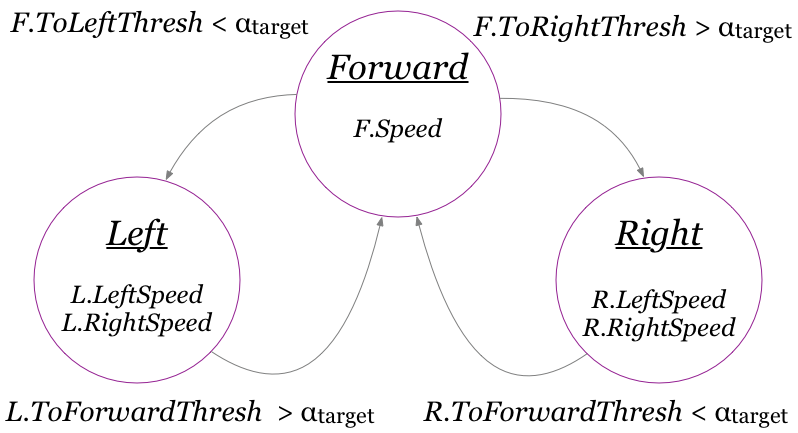
\includegraphics[width=0.3\textwidth,valign=c]{figures/3-adabot/FSM-direction.png}%
        \vphantom{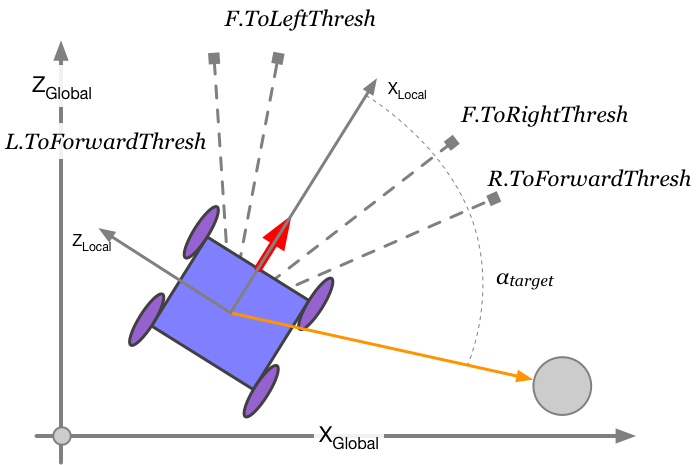
\includegraphics[width=0.3\textwidth,valign=c]{figures/3-adabot/scene.png}}%
    }
    \hfil
    \subfloat[Strut Extension Control]{%
        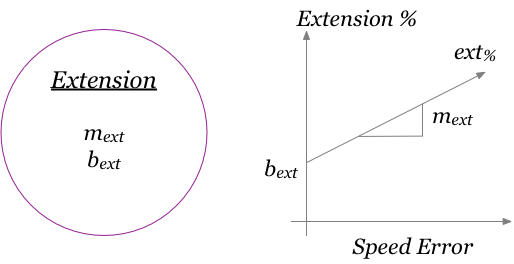
\includegraphics[width=0.2\textwidth,valign=c]{figures/3-adabot/FSM-strut.png}%
        \vphantom{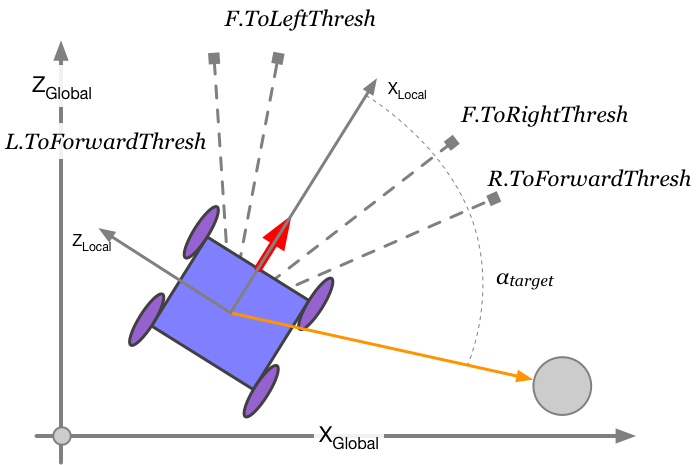
\includegraphics[width=0.3\textwidth,valign=c]{figures/3-adabot/scene.png}}%
    }
    \hfil
    \subfloat[Environment Diagram]{%
        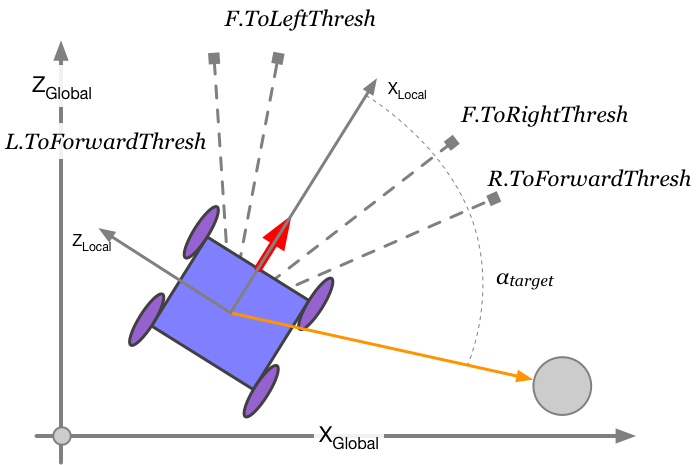
\includegraphics[width=0.3\textwidth,valign=c]{figures/3-adabot/scene.png}%
        \vphantom{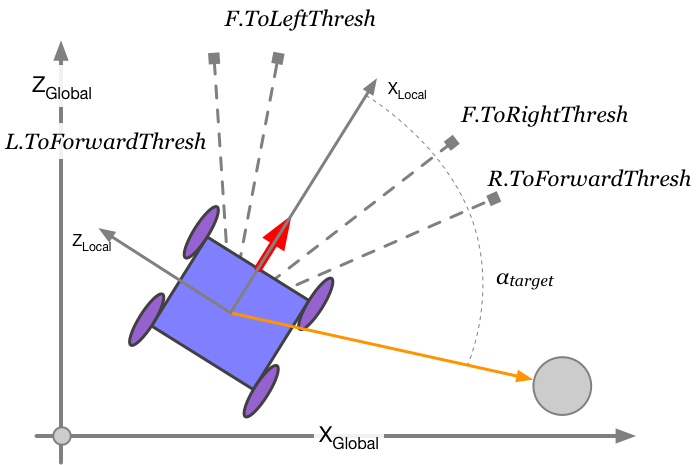
\includegraphics[width=0.3\textwidth,valign=c]{figures/3-adabot/scene.png}}%
    }

    \vspace{-0.08in}

    \caption{(a) The FSM controlling the direction of the robot, (b) the single state controlling wheel struts, and (b) a diagram depicting the angles used to trigger transitions between states.}
    \label{fig:fsm}

    \vspace{-0.1in}

\end{figure*}



The second action, handling the wheel struts, is accounted for by the state shown in the lower part of \figref{fig:fsm}(a).
%
This state calculates the expected linear ($v_{\mathit{UGV}}$) and angular ($\omega_{\mathit{UGV}}$) speed using a simple differential drive model:

\vspace{-0.08in}

\begin{align}
  v_{\mathit{UGV}} &= \frac{V_r + V_l}{2},\\
  \omega_{\mathit{UGV}} &= \frac{V_r - V_l}{\mathit{TrackWidth}}
\end{align}

\noindent
where $V_r$ and $V_l$ are the left and right wheel linear velocities (depending on the left and right wheel rates, described below, as well as $\mathit{WheelRadius}$), respectively, and $\mathit{TrackWidth}$ represents the distance between wheels on the same axle line (front or rear axles).
%
As we are dealing with a noise-free, idealized simulation, this differential drive model has shown to be very accurate.
%
It compares the expected speed to the actual speeds of the device, which are known exactly in simulation and can be measured accurately using an overhead camera setup in physical experiments, to calculate the scaled (between 0 and 1) absolute error values $v_{\mathit{UGV}_e}$ and $\omega_{\mathit{UGV}_e}$.
%
These errors values are filtered using exponential smoothing and then used in the following equations to calculate the extension amount of all struts:

\vspace{-0.2in}

\begin{align}
    \mathit{ext}_v &= m_{\mathit{ext}} \cdot v_{\mathit{UGV}_e} + b_{\mathit{ext}},\\
    \mathit{ext}_\omega &= m_{\mathit{ext}} \cdot \omega_{\mathit{UGV}_e} + b_{\mathit{ext}},\\
    \mathit{ext}_\% &= \max[\mathit{ext}_v, \mathit{ext}_\omega],\\
    \mathit{ext} &= \mathit{MAXEXT} \cdot \mathit{ext}_\%
\end{align}

\noindent
where $\mathit{ext}_v$ and $\mathit{ext}_\omega$ denote the extension amount calculated due to the linear and angular speed values, respectively. These two values are calculated using a linear equation with a configurable slope ($m_{\mathit{ext}}$) and intercept ($b_{\mathit{ext}}$).
%
The final extension amount is based on the maximum of these two values, and is calculated as a percentage of the maximum possible extension ($\mathit{MAXEXT}$).
%
In essence, the struts will be extended an amount that is linearly proportional to the current error in speed.
%
Thus, when Adabot encounters an obstacle that blocks it from moving according to the differential drive model it will extend the struts in an effort to climb over any obstacles.
%
\tblref{tbl:params-fsm} shows all configurable parameters for the FSM. Aside from the first two rows, each name in the table takes the following form: a capital letter representing a state in \figref{fig:fsm}(a) (\textbf{F}\emph{orward}, \textbf{L}\emph{eft}, or \textbf{R}\emph{ight}), followed by a period, followed by either an angular wheel rate or a angle threshold value also found in \figref{fig:fsm}(a).

\begin{table}[hb]
    \centering
    \caption{Adabot FSM Parameters}
    \label{tbl:params-fsm}
    \begin{tabular}{@{}ll@{}}
        \toprule
        \textbf{Name} & \textbf{Range}\\
        \midrule
        $m_{\mathit{ext}}$ & \numrange{0}{1}\\
        $b_{\mathit{ext}}$ & \numrange{0}{1}\\
        $F.Speed$ & \numrange{0}{20}~\si{\radian\per\second} \\
        $F.ToLeftThresh$ & \numrange{0}{90}\si{\degree}\\
        $F.ToRightThresh$ & \numrange{-90}{0}\si{\degree}\\
        $L.LeftSpeed$ & \numrange{-20}{20}~\si{\radian\per\second} \\
        $L.RightSpeed$ & \numrange{-20}{20}~\si{\radian\per\second} \\
        $L.ToForwardThresh$ & \numrange{0}{90}\si{\degree}\\
        $R.LeftSpeed$ & \numrange{-20}{20}~\si{\radian\per\second} \\
        $R.RightSpeed$ & \numrange{-20}{20}~\si{\radian\per\second} \\
        $R.ToForwardThresh$ & \numrange{-90}{0}\si{\degree}\\
        \bottomrule
    \end{tabular}
\end{table}


For this study we decided to use this single, simple state (based on just to configurable values) to reduce the number of factor that must be considered while comparing the FSM to the ANN.
%
In future work we plan to extend this FSM to handle more complex tasks and exhibit more complex dynamics.
%
One final, important note regarding Adabot's control system. To reduce vibration and potential damage to the wheel struts, the maximum angular rate of the wheels is linearly scaled down from 20~\si{\radian\per\second} to 4~\si{\radian\per\second} when the struts are fully extended.


\vspace{0.1in}
\noindent
\textbf{ANN Control}
As an alternative to the FSM controller, we evolve an ANN for the same task.
%
The neural network receives three inputs: (1) $\alpha_{\mathit{target}}$ scaled between 0 and 1, (2) $v_{\mathit{UGV}_e}$, and (3) $\omega_{\mathit{UGV}_e}$.
%
Essentially, the ANN is given the same information as the FSM, and produces the same three output values (left and right wheel rates and an extension amount).
%
For the sake of analyzing the evolved networks, we chose to make the ANN as simple as possible. Thus, the network is feed-forward and it does not include any hidden nodes.
%
The genome for our ANN includes 13 values: one integer value representing the activation function (logistic, hyperbolic tangent, or the rectified linear unit) and 12 values for the neural network weights (three inputs plus one bias times three outputs).



% \subsection{Evolution}
% \paragraph{Evolution}
\vspace{0.1in}
\noindent
\textbf{Evolution}
%
For this study, we employ the Covariance Matrix Adaptation Evolution Strategy (CMA-ES)~\autocite{Hansen.2003.EC.CMAES}.
%
In particular, we use the Python implementation, pycma\footnote{https://github.com/CMA-ES/pycma}, developed by the original author of CMA-ES.
%
CMA-ES was chosen as it works well on real-valued problems and has support for handling integer values in the genome (as is the case for $\mathit{ExtCount}$).
%
Although we experimented with several of the configurable parameters, we did not notice any positive results when changes values from their defaults.

\section{Discussion and Results}
\label{sec:results}

In this section we provide our results from evolving the Adabot.
%
Specifically, we evolved the Adabot in two environments (with and without obstacles) and with two different controllers (the FSM defined in \secref{sec:adabot} and an ANN). Each of these four experiments is repeated 20 times.
%
Finally, we discuss principles that can be learned from these experiments.


\subsection{Fitness Calculations}

% As discussed in the previous section, the goal of our robot is to visit a set of coordinates (way-points) in sequence.
%
Here, Adabot's goal is to visit a set of coordinates (way-points) in sequence.
%
During a single simulation, the device has 30 seconds to visit \textbf{four} predefined way-points, but the simulation will terminate as soon as the fourth way-point is reached.
%
Fitness is calculated as follows:

\vspace{-0.08in}

\begin{align}
    f &= 2w + (1-\frac{\min[d, d_\mathit{max}]}{d_\mathit{max}}) + \frac{(30 - t)}{30}
\end{align}

\noindent
where $w$ represents the number of way-points reached, $d$ and $d_\mathit{max}$ denote the distance to the next way-point and a scaling factor for distances, respectively, and $t$ denotes the time at the end of the evaluation.
%
This function is meant to provide a smooth gradient for generating controllers that quickly navigate to all way-points in order.
%
The first part of the equation ensures that the CMA-ES algorithm heavily favors any controller that reaches even a single way-point; values for this component range from 0 to 8.
%
Next, a distance component is added to reward any solutions that drive near its next way-point. This is particularly useful at the beginning when solutions are randomly generated.
%
The distance component results in a value scaled between 0 and 1.
%
Since the simulation ends once all four way-points have been reached, the time component will be a value between 0 (zero time remaining) and 1 (all four way-points are reached in an instant).
%
The time component is meant to favor any controllers that solve the task quickly.
%
Thus, the maximum possible fitness is 10.


\subsection{Evolution Without Obstacles}

In our first experiment, \emph{FSM-0-1}, we evolve the fifteen parameters found in Tables~\ref{tbl:params-physical} and~\ref{tbl:params-fsm} in an environment without obstacles.
%
The naming scheme for our experiments indicates the controller type (\emph{FSM} or \emph{ANN}), the maximum number of potential obstacles (0 or 40), and the number of trials per fitness evaluation (1 or 2).
%
Plots of fitness vs iteration are show in \figref{fig:fitness-vs-iteration} (this figure shows the fitness values for all four experiments).
%
In this first experiment, there are zero obstacles and therefore the environment will always be the same. In later experiments, each fitness evaluation includes two trials with randomly generated obstacles.
%
As shown in the figure, in all replicate trials the Adabot reaches all four way-points in approximately 10 seconds, which corresponds to a fitness value of 9.7.
%
The population quickly converges on a final value, likely because this experiment was seeded with a hand-designed set of parameters known to achieve good results; the evolved results, however, quickly outperform the hand-chosen values.
%
This experiment serves as a convenient baseline with which the others can be compared.

\begin{figure}[!ht]
    \centering

    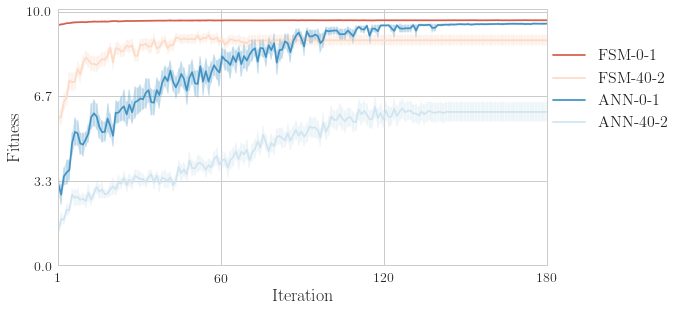
\includegraphics[width=\columnwidth]{figures/4-results/fitness.png}

    \vspace{-0.1in}

    \caption{Fitness plots for the maximum fitness found in each of the four experiments. The shaded regions indicate confidence intervals of one standard deviation from the mean for the 20 replicated trials of each experiment. The maximum possible fitness is 10 and any fitness value above 2 means that UGV was able to reach at least one way-point.}
    \label{fig:fitness-vs-iteration}

    \vspace{-0.05in}
\end{figure}


The second experiment, denoted \emph{ANN-0-1}. also reaches a fitness value of 9.7, which shows that the an ANN can effectively perform the task of navigating the robot to a sequence of points.
%
For this experiment, 17 total parameters were evolved: the four physical characteristics listed in \tblref{tbl:params-physical} and the 13 ANN parameters discussed in the previous section.
%
Although both of these experiments reach the same final fitness value, an examination of \figref{fig:fitness-vs-iteration} shows that the ANN result takes longer to evolve--roughly 120 iterations compared with less than 10 iterations for the FSM.
%
This can be explained by the lack of a seed controller and the fact that, unlike an FSM, an ANN must learn the entire solution from scratch.


\figref{fig:0-1-best-trajectories} depicts the trajectories taken by the best performing controllers from these two experiments.
%
Although these trajectories look similar, there is one key difference: the ANN actively controls only one wheel. The FSM, on the other hand, occasionally rotates in both directions by turning its left and right side wheels in opposite directions.


\begin{figure}[!ht]
    \centering

    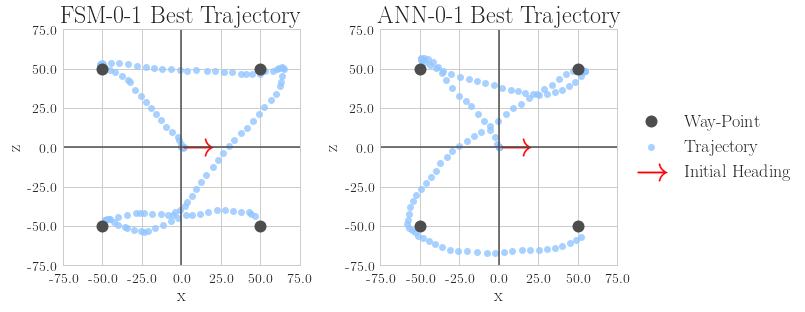
\includegraphics[width=\columnwidth]{figures/4-results/0-1-best_trajectories.png}

    \caption{Trajectories of the best evolved individual for the first two experiments: FSM-0-1 and ANN-0-1. No obstacles were present for these trajectories.}
    \label{fig:0-1-best-trajectories}
\end{figure}


% This tactic can be more easily seen in \figref{fig:ANN-0-1-best-speed}.
\figref{fig:ANN-0-1-best-speed} shows the wheel speeds for the best FSM and ANN controllers.
%
% This figure shows that t
The evolved ANN perpetually sets the right wheel to its maximum speed.
%
The ANN moves forward by setting its left wheel to the same value, and turns by making the left wheel rotate in the opposite direction.
%
Effectively, the ANN can only turn left, however, this is not a problem for the relatively simple task at hand.



\begin{figure}[!ht]
    \centering

    \subfloat[]{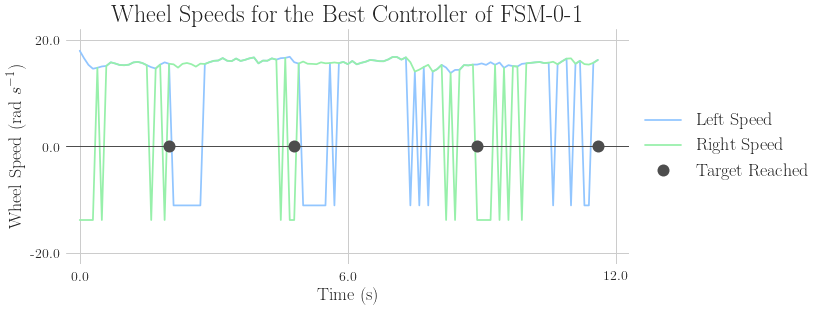
\includegraphics[width=\columnwidth]{figures/4-results/FSM-0-1-best_speed.png}}
    \hfil
    \subfloat[]{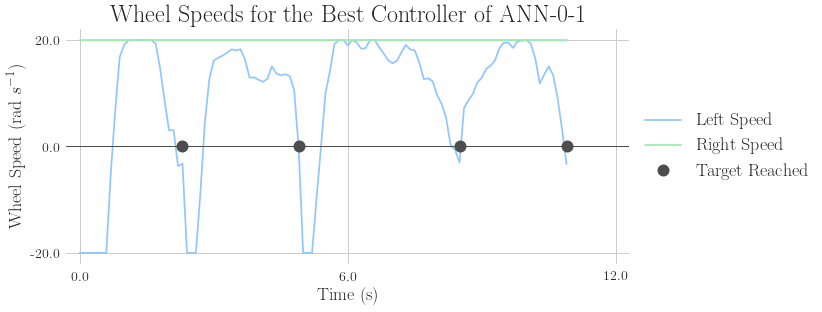
\includegraphics[width=\columnwidth]{figures/4-results/ANN-0-1-best_speed.png}}

    \caption{Left and right wheel speeds for the best evolved solutions for \emph{FSM-0-1} (a) and \emph{ANN-0-1} (b).}
    \label{fig:ANN-0-1-best-speed}

    \vspace{-0.1in}
\end{figure}


\figref{fig:0-1-best-params} provides a comparison of the fitness values and evolved physical characteristics for these two experiments.
%
This figure only shows results for the combined final populations of all replicate experiments.
%
From this figure, we can establish what will be good physical characteristics for the Adabot when it does not face any obstacles.
%
Specifically, \emph{WheelBase} and \emph{TrackWidth} should be 8.5~\si{cm} and 11.5~\si{cm}, respectively, \emph{WheelRadius} should be 3~\si{cm}, and each wheel should have at least 4 wheel struts (\emph{StrutCount}).


\begin{figure}[!ht]
    \centering

    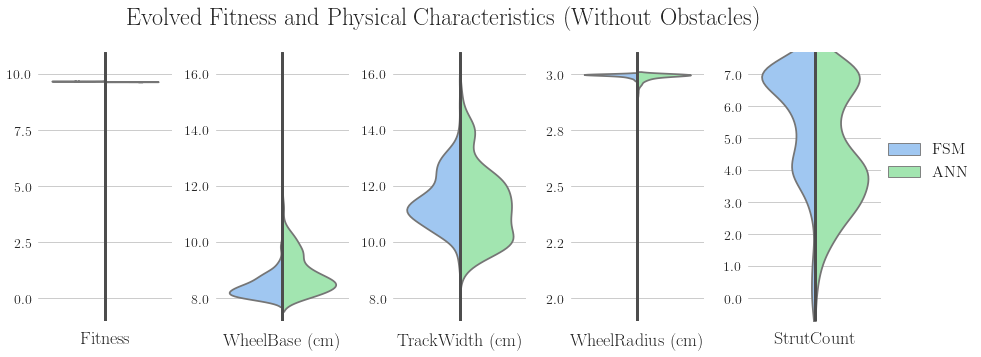
\includegraphics[width=\columnwidth]{figures/4-results/0-1-best_params.png}

    \caption{Distributions for the evolved fitness values and physical characteristics for the combined final populations of the \emph{FSM-0-1} (left side) and \emph{ANN-0-1} (right side) experiments. The y-axis limits are the parameter limits allowed during evolution.}
    \label{fig:0-1-best-params}

    \vspace{-0.2in}

\end{figure}


Finally, \figref{fig:FSM-best-params}(a) plots the distributions for all evolved FSM parameters.
%
It is worth noting that neither the evolved FSMs or ANNs extend the struts.
%
This results is not unexpected as any extension would result in a reduced speed (due to the scaling mentioned in \secref{sec:adabot}), and the struts are not needed when obstacles are not present.
%
Also of interest is the evolved symmetry of the FSM.
%
Specifically, the threshold values and speeds evolved for the \emph{Left} and \emph{Right} states are nearly perfect mirror images of each other.


\begin{figure*}[!ht]
    \centering

    % \subfloat[]{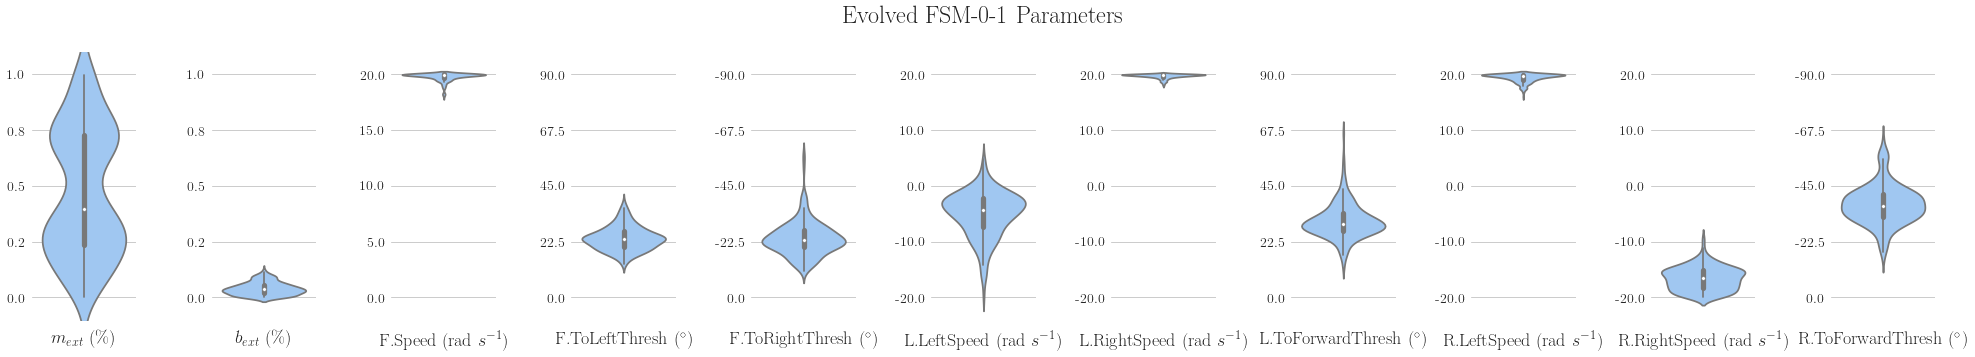
\includegraphics[width=\textwidth]{figures/4-results/FSM-0-1-best_params.png}}
    % \hfil
    % \subfloat[]{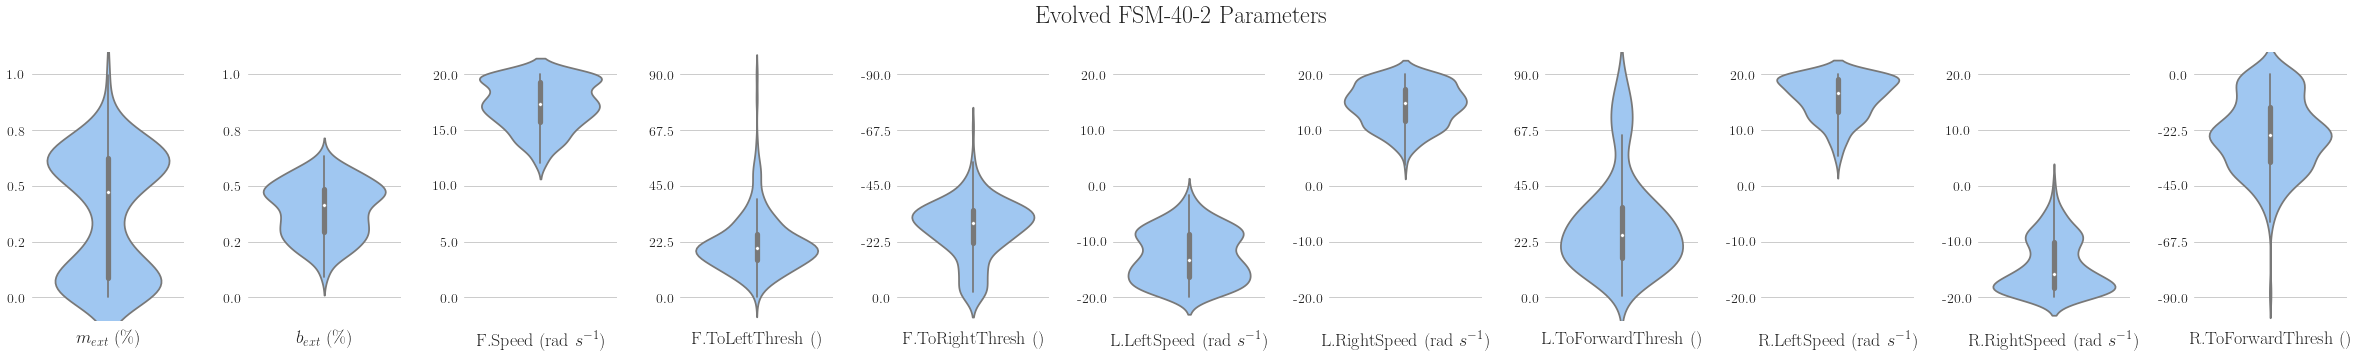
\includegraphics[width=\textwidth]{figures/4-results/FSM-40-2-best_params.png}}

    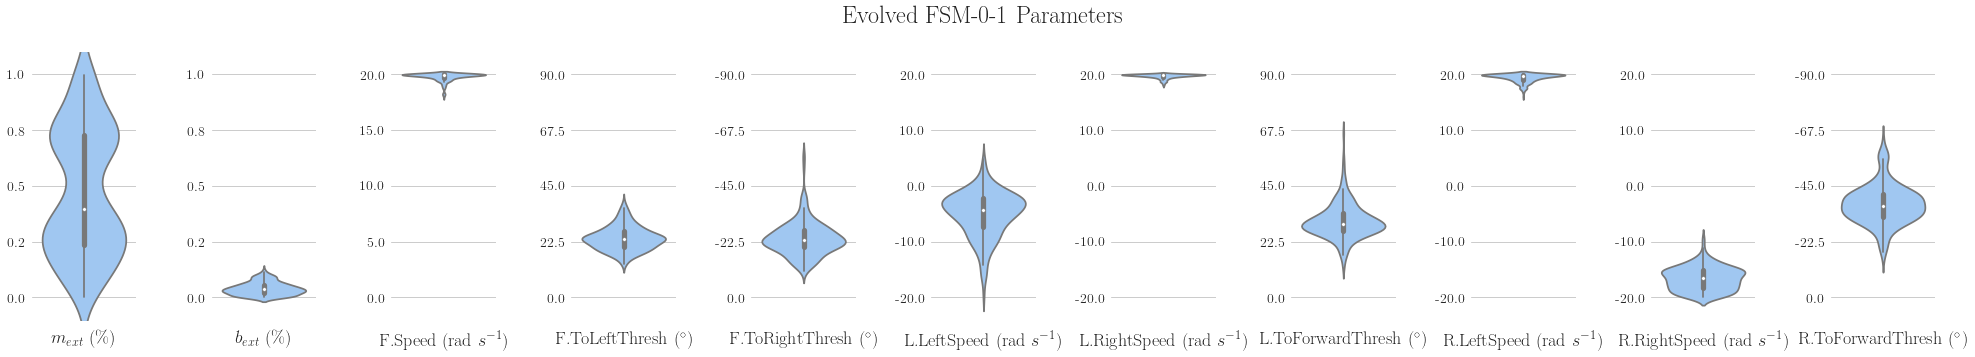
\includegraphics[width=\textwidth]{figures/4-results/FSM-0-1-best_params.png}

    % \caption{Distributions for all evolved FSM parameters for the \emph{FSM-0-1} and \emph{FSM-40-2} experiments.}
    \caption{Distributions for all evolved FSM parameters for the \emph{FSM-0-1} experiment.}
    \label{fig:FSM-best-params}
\end{figure*}


\subsection{Evolution With Obstacles}

% Best BNN
% '30 40 0 0.08218 0.1193 0.02994 5 0 3.983 3.718 -0.6273 -3.185 -0.1238 -0.6903 1.984 3.977 2.171 2.209 3.999 -0.2371'

% Best FSM
% '30 40 0 0.09734 0.1259 0.02998 6 0.4915 0.3365 0.8207 0.8632 -0.377 -0.7851 0.9327 0.7227 0.6914 -0.9314 -0.6232'

The final two evolutionary experiments are referred to as \emph{FSM-40-2} and \emph{ANN-40-2}.
%
These experiments differ from the previous two in two respects. First, each fitness value is calculated as the average of two trials (where each trial lasts at most 30 seconds), and second, each fitness trial occurs in an environment with at most 40 randomly generated obstacles.
%
Utilizing multiple trials during fitness evaluations improves the robustness of the evolved results~\autocite{Ruud.SSCI.EvoLearn.2016}.
%
The fitness plots for these experiments appear in \figref{fig:fitness-vs-iteration}.
%
Of note is that the ANNs evolved with obstacles have a greatly reduced maximum fitness. A few individuals achieve a fitness above 9, however, we found that this was only when the randomly generated environment did not pose much difficulty.
%
We have provided videos for the highest fitness individuals from both experiments\footnote{\emph{FSM-40-2} example behavior: \url{https://youtu.be/VXnrwwpE598}}\footnote{\emph{BNN-40-2} example behavior: \url{https://youtu.be/q8PFqQps5e4}}.


% After reviewing the distributions in Figures~\ref{fig:0-1-best-params} and~\ref{fig:40-2-best-params}
Similar to \figref{fig:0-1-best-params}, \figref{fig:40-2-best-params} shows the distributions for the evolved physical characteristics.
%
The values found in these distributions indicates that the presence of obstacles does not have a drastic affect on the evolution of physical characteristics.
%
At first this was unexpected, however, analyzing these values (and visualizing their resulting behaviors) reveals a few basic principles:
(1) for a skid steer robot it is important for the \emph{WheelBase} to be less than the \emph{TrackWidth} (this will reduce the amount of \emph{skidding} and improve controllability),
(2) to maximize velocity \emph{WheelRadius} should be maximized (since we are evolving wheel angular rate a larger wheel will result in a higher velocity), and
(3) as long as the number of struts is greater than 4 the system will be able to navigate the generated environments.
%
The first and second principles match results that we have seen on the physical prototype, and we intend to investigate the third principle in the near future.
%
This leaves us with control being the most important factor in navigating obstacles.


\begin{figure}[!ht]
    \centering

    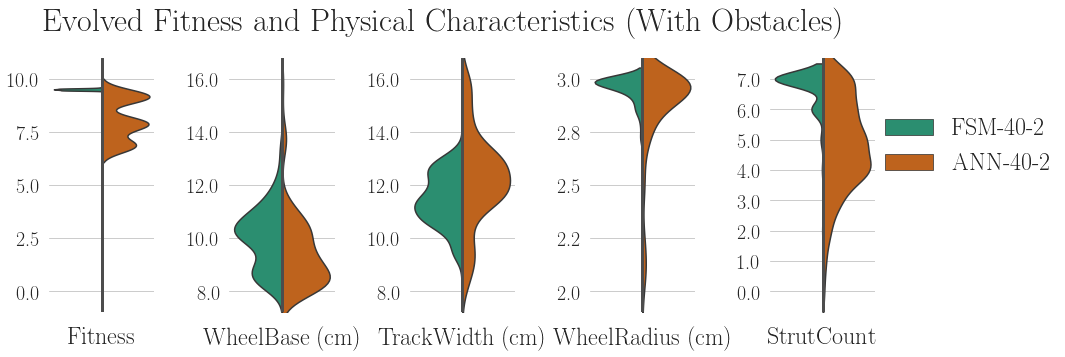
\includegraphics[width=\columnwidth]{figures/4-results/40-2-best_params.png}

    \vspace{-0.07in}

    \caption{Distributions for the evolved fitness values and physical characteristics for the combined final populations of the \emph{FSM-40-2} (left side) and \emph{ANN-40-2} (right side) experiments. The y-axis limits are the parameter limits allowed during evolution.}
    \label{fig:40-2-best-params}

    \vspace{-0.2in}

\end{figure}



While the physical characteristics are similar between the two sets of experiments, control strategies have been changed to handle the obstacles.
%
\figref{fig:40-2-best-speed} shows the control patterns for two solutions randomly selected from the best performing individuals of the \emph{FSM-40-2} and \emph{ANN-40-2} experiments.
%
Note that since environments are randomly generated, even though the evolved ANN does not reach all four way-points for this test, it does not mean that it did not do so during fitness evaluation.
%
The most important feature of the plots in \figref{fig:40-2-best-speed} are that the evolved controllers are operating at a reduced speed.
%
% Examining the evolved values in \figref{fig:FSM-best-params} shows that for at least the \emph{FSM-40-2}, the evolved speeds are still near the maximum allowed value.
%
Examining the evolved FSM values , we see that nearly identical values are discovered for all parameters except $b_{\mathit{ext}}$
(a set of distributions similar to \figref{fig:FSM-best-params} has been omitted to save space).
%
In the experiment with no obstacles, $b_{\mathit{ext}}$ was consistently set to a value near zero, however, for this experiment $b_{\mathit{ext}}$ was set to 0.45.
%
A higher value for $b_{\mathit{ext}}$ results in the struts always being extended (even when no obstacle has been encountered).
%
Thus, the cause of the slower behavior is that the controllers are using the struts to improve mobility in the face of obstacles.
%
% This can also be seen by looking at the evolved values for $b_{\mathit{ext}}$, without obstacles this value is near zero, and with obstacles this value is closer to 0.45.




\begin{figure}[!ht]
    \centering

    \subfloat[]{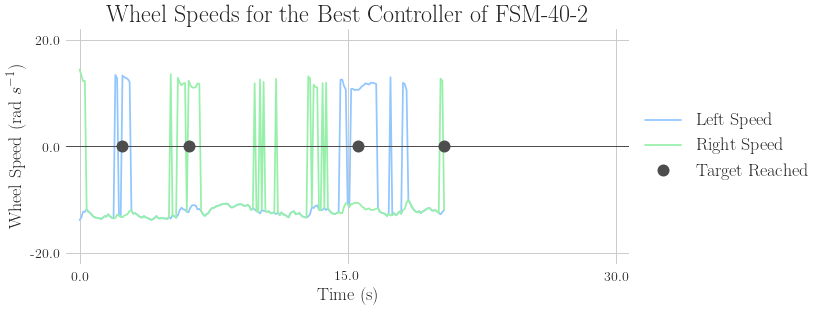
\includegraphics[width=\columnwidth]{figures/4-results/FSM-40-2-best_speed.png}}
    \hfil
    \subfloat[]{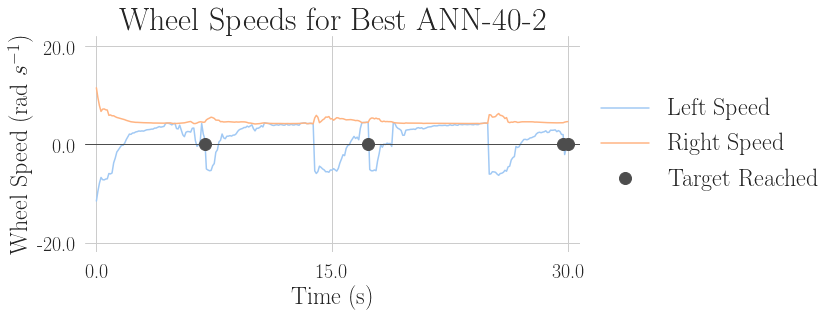
\includegraphics[width=\columnwidth]{figures/4-results/ANN-40-2-best_speed.png}}

    \vspace{-0.1in}

    \caption{Left and right wheel speeds for the best evolved FSM (a) and ANN (b) in a randomly generated environment that includes obstacles.}
    \label{fig:40-2-best-speed}

    \vspace{-0.1in}

\end{figure}





The final set of evolved parameters to examine is those of the neural network.
%
Directly examining the evolved weights provides only a limited view of the resulting behavior. Likewise, comparing each input's effect on each output in isolation also obscures analysis.
%
For example, some output values are only active when some combination of multiple input values is provided.
%
Thus, in \figref{fig:ANN-40-2-best-ann-map} we provide all pairwise heat-maps for all inputs and outputs.
%
These heat-maps were generated using a parameter sweep over all possible input combinations. Each square represents the average output value given the two input values on the x- and y-axes and all possible values for the remaining input.
%
Looking at the second and third rows in this figure we can see that for any combination of input values the right wheel is always rotating at a constant forward speed and the struts are always fully extended, respectively.
%
As was the case for the \emph{ANN-0-1} experiment, all navigation is handled by driving the left wheel at different speeds.
%
Examining the first row shows that the left wheel's speed has a linear relationship with all three neural network inputs.
%
As any of the inputs are increased, so to does the left wheel speed.


In both experiments including obstacles, the evolved controllers extended the struts and never fully retracted them.
%
However, there is a clear advantage to retracting the struts: the robot has a higher maximum allowed speed.
%
Thus, it is likely an issue with using the differential drive model to calculate the error.
%
We have identified two sources of error with simple model: (1) it does not take into account that when the struts are extended the wheel has a larger effective radius, and (2) the model does not take into account the noisy nature of a skid steering and extended struts.


\begin{figure}[!ht]
    \centering

    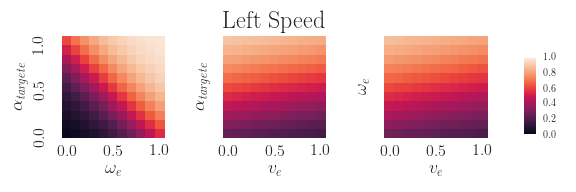
\includegraphics[width=\columnwidth]{figures/4-results/ann_map.png}

    \caption{Heat-maps showing the relationship between input and output for the best evolved ANN. For example, the first row represents the output wheel rate for the left wheels, a light shade indicates that the wheel is at its maximum forward rate, and a dark color indicates that it is at its maximal reverse rate. All input and output values are scaled between 0 and 1.}
    \label{fig:ANN-40-2-best-ann-map}

    \vspace{-0.08in}

\end{figure}


To summarize our findings regarding the optimization of the Adabot system:

\begin{enumerate}

\item Similar physical characteristics are optimal with and without obstacles in the environment.

\item The speed of the left and right wheels should have a linear relationship with $\alpha_{\mathit{target}}$ (rather than a discrete relationship as is the case with the current FSM).

\item The task can be solved by controlling only a single wheel, though, this is likely not a desirable trait. In future work, we plan to add an evolutionary pressure so that the evolved ANNs turn in both directions.

\item Controlling the strut will require a more complex model of the robots dynamics. Once the struts are extended, it is difficult to discern when they can be retracted.

\end{enumerate}

Taking these observations into account, we developed a hybrid two-state controller. The controller is in \emph{LeftState} when $\alpha_{\mathit{target}}$ is greater than zero and in \emph{RightState} otherwise. Equations for these states are as follows:

\vspace{-0.1in}

\begin{align}
    \alpha_\mathit{scale} &= 2\cdot(1 - \frac{\alpha_{\mathit{target}}}{\pi}) - 1\\
    \mathit{LeftState}_\mathit{left} &= \mathit{MAXRAD} \cdot \alpha_\mathit{scale}\\
    \mathit{LeftState}_\mathit{right} &= \mathit{MAXRAD}\\
    \mathit{RightState}_\mathit{left} &= \mathit{MAXRAD}\\
    \mathit{RightState}_\mathit{right} &= -\mathit{MAXRAD}\cdot \alpha_\mathit{scale}
\end{align}

\noindent
where $\alpha_\mathit{scale}$ is $\alpha_{\mathit{target}}$ scaled between 1 and -1 (the sign is flipped). This simple hybrid controller is able to visit all way-points in 9.9 seconds, which is one tenth of a second faster than the evolved controllers reported above. The controller also works well in the presence of obstacles when the struts are extended 10\%. Overall, this hybrid controller provides a smoother motion and good performance. For future work, we intend to evolve this hybrid controller along with a more sophisticated approach to handling strut extension.

\section{Conclusion}
\label{sec:conclusion}

UGVs are becoming more prevalent. Likewise, their envisioned environments are becoming more dynamic and varied.
%
We have evolved a UGV so that it is better able to handle obstacles of varying sizes.
%
Specifically, we compared and analyzed FSM and ANN controllers with and without obstacles in the environment.
%
Comparing these two techniques enabled us to propose a new hybrid controller that incorporates the advantages of both.
%
Although a direction controller was straightforward to optimize, the complex dynamics associated with climbing over obstacles makes it more difficult to design a controller for extending the Adabot' struts.
%
Our future work will focus on optimizing the hybrid controller and investigating different techniques for extending the struts.


% Talk about more complex neural networks (recurrent, hidden nodes, etc.).

% More complex tasks (sequential tasks lexicase).

\section{Acknowledgements}

This work was supported by NSF grant No.\ PHY-9723972.


% \begin{acks}

% The authors would like to thank...

% \end{acks}


\bibliographystyle{plainnat}
\bibliography{references/refs}

\end{document}
